\chapter{}
As sempre lembradas festas de fim de ano da nossa família alcançaram seu apogeu quando as tias se mudaram para a sua nova casa, na Rua Carlos Gomes, por volta de mil novecentos e cinquenta e cinco ou seis, por aí.
A casa tinha um grande quintal calçado de pedras e uma cozinha nos fundos, equipada com um belo fogão a lenha.
Uma semana antes do Natal, quando os tios do Rio anunciavam sua iminente chegada, sob o comando do tio Bepe, uma grande barraca de lona era erguida no local.
Ao comprido dessa tenda, com tábuas e cavaletes, uma mesa extensa era preparada para receber umas cinquenta pessoas, pelo menos.
Então, tinha início a trabalheira.
Da fazenda, Tio Totó e Tio Zé traziam engradados de frangos, leitoas e cabritos, além de quartos de boi.
Papai se encarregava das bebidas.
Tia Yolanda vinha reforçar a brigada da cozinha aonde a lida ia do amanhecer ao anoitecer, sem parar.
Os animais eram abatidos, limpos, esquartejados e postos em vinha d’alhos.
Panetones, canarícoles, estrufules, bolos de especiarias, compotas, espalhavam seu perfume por todo o quarteirão.
Quilos de massa de trigo eram sovados pelos poderosos braços da Tia Glória, para fazer os pães e o macarrão que seriam consumidos em quantidades industriais.
Grosas de tomate maduro cozinhavam em panelões por horas a fio para fazer o molho do espaguete, do nhoque, dos raviólis, dos fuziles trabalhosamente enrolados um a um, com a ajuda de arame grosso.
Um enorme barril de chope era posto a gelar e era apenas o primeiro dos quatro ou cinco a serem esgotados até o início do novo ano.

Assim que os tios do Rio e respectivas famílias estacionavam à porta, a grande comemoração tinha início.
Meus avós maternos, assim como todos os outros parentes araraquarenses e os parentes dos parentes, noivos, namorados, amigos dos amigos, a partir desse momento tomavam na própria casa apenas o café da manhã.
Para o almoço, seguiam para a casa das tias e de lá só saiam no princípio da madrugada, gratos e empanzinados pela farta, alegre e incansável hospitalidade delas.

Hoje, não vejo como seria possível promover uma comilança daquela envergadura.
Contando, ninguém acredita.
Mas a verdade é que naqueles tempos em que não se discutia triglicérides e colesteróis, aquela gente entregava-se desbragadamente ao prazer de comer sem culpa e esse fato contribuía com parte considerável do sucesso da festa.
As tias percorriam léguas do fogão à mesa e de volta ao fogão, levando travessas cheias e trazendo de volta as vazias para enchê-las novamente.
Frituras crocantes, assados envernizados de gordura, massas nadando em molhos, doces lambuzados de mel, de calda de açúcar, de cremes, nada intimidava os animados convivas sempre capitaneados pelo Pepone cujo perfil, lá pelas tantas, começava estranhamente a assumir o contorno do barril de chope que ele cuidava de esvaziar em grandes e entusiasmados sorvos, dignos de um guerreiro viking.


Por volta da meia-noite da véspera do Natal, as tias desapareciam momentaneamente do cenário, não sem antes abastecer a mesa mais uma vez, para que ninguém ficasse desassistido enquanto elas corriam até a Matriz para a Missa do Galo.
Raras vezes alguém deu pela falta delas.


Início da madrugada, Pepone, já liberto de todas as amarras, dava início aos discursos e aos brindes.
Aos \textit{hip}, \textit{hip}, \textit{hurras!} e vira-viras que acompanhavam a competente ingestão de mais alguns canecos de chope, todos os presentes recebiam vivos agradecimentos pela honrosa presença e eram postos a par da tradição de hospitalidade que distinguia os Filpi desde Novi Veglia, na distante Salerno, até o momento em curso.
Nessa nostálgica trajetória, Tio Bepe, flutuando nos vapores do chope, ia se emocionando progressivamente até chegar à lembrança da ``nossa santa mãe'', referência que sempre fazia chegar lágrimas aos olhos de todos os machos da família, orador incluído.
Apenas meu pai se continha, consciente da expressão zombeteira que assomava ao rosto da minha mãe, sempre que os cunhados se punham a canonizar ``aquela virago''.
Nesta altura, Tio Totó intervinha e tomava a palavra, coisa que ele perceptivelmente desejava fazer desde o início, afinal o político ali era ele, e completava a elegia com merecidas homenagens ``às nossas santas {\large\bfseries ermãs}'', como ele dizia.
Mais alguns \textit{hip-hurras}, aplausos e Tio Bepe, já recuperado do surto emocional, mas não da bebedeira, bradava seu grito carnavalesco predileto -- \textit{“Alalaô, ooô, ooô! Mas que calor, ooô,ooô!”}, -- e arrastando todo mundo para o cordão de que ele assumia o comando logístico–musical, punha-se a evoluir pela casa até cair semi-desmaiado em algum canto.
Houve um ano em que se superando, ele concluiu sua performance exibindo-se num sapateado de elefante amestrado sobre o barril vazio, para assombro dos circunstantes.


\begin{figure}[H]
\centering
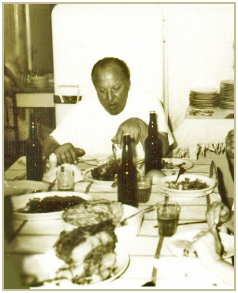
\includegraphics[width = 0.6\linewidth]{10/pepone-natal.png}
\caption{Pepone presidindo a mesa de Natal.}
\end{figure}

Ano após ano, ainda que soubéssemos que o enredo era sempre o mesmo, por nada perdíamos as festas de fim de ano na casa das tias.
Enquanto as quatro juntas puderam agüentar aquela verdadeira maratona culinária com a mesma disposição e a mesma generosa alegria, ninguém ali pensou em desfrutar o final do ano em outro lugar.

Quando Tia Glória, a última das irmãs a ir-se deste mundo, estava próxima da morte, eu a visitava diariamente.
A tia já há anos vivia imobilizada na sua poltrona, mas continuava lúcida e, nesse final de vida, tornara-se sábia, não obstante ter passado a maior parte dos seus oitenta e dois anos à beira de um fogão.
Numa tarde telefonou-me, pedindo que especialmente naquele dia não deixasse de ir vê-la, pois tinha um pedido a fazer.
Fui.
A tia estendeu-me um caderno onde estavam anotadas as receitas que por dezenas de anos tinham feito a fama da sua cozinha.
Queria que eu a ajudasse a selecionar aquelas mais fáceis e saborosas para reuni-las num livrinho que pudesse enviar às sobrinhas do Rio.
\textit{``-- Você pode fazer isso bem organizadinho no seu computador, não pode?''}, quis saber ela.

Disse que podia.
Então, ela justificou o pedido mais ou menos assim:
\textit{``-- Filha, você e suas primas daqui conviveram conosco, aprenderam a cozinhar direitinho e sabem da importância de reunir a família em torno de uma mesa, partilhando uma comida bem feita, gostosa.
Foi assim que mantivemos nossa gente unida por tanto tempo.
Tem quem possa achar que eu fui infeliz, dedicando a minha vida toda a cozinhar para vocês.
Mas hoje, olhando para trás, penso que essa foi uma missão que me destinaram e sou feliz por tê-la cumprido direito.
Fico preocupada com essas sobrinhas lá longe, vivendo numa cidade tão grande e tão difícil.
Sabe-se lá se têm tempo de preparar alguma coisa para os maridos e os filhos.
Essas receitas elas poderão fazer em poucos minutos, sem perigo de errar.
Todas foram testadas muitas vezes por mim.
Assim morro sossegada, sabendo que elas também poderão reunir sua gente em volta da mesa, como sempre foi na nossa família.
Você pode mandar junto com o livrinho uma carta, explicando isso tudo?''}

\begin{figure}[H]
\centering
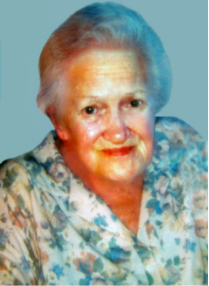
\includegraphics[width = 0.6\linewidth]{10/tia-glória.png}
\caption{Tia Glória aos 81 anos.}
\end{figure}

E foi dessa maneira que, naquela tarde, ajudei Tia Glória a lavrar o que, me parece, foi seu único testamento, ou, melhor dizendo, sua confissão de fé.
 
